\documentclass{report}
\usepackage{green_buddhism}
\title{Green Buddhism: A Programmer's Religion}
%\subtitle{Enjoying a life of liberty}
\author{Logan Streondj elspru@zeroid.bit}
\begin{document}

\part{Galaxy Domain Strategy}

\section{Origination}
\label{origination}
\begin{table}
\begin{tabular}{l l} 
  no colour & black \\
  no sound & quiet \\
  no emotion & content \\
  no motion & stopped \\
  no number & zero \\
  no temperature & zero kelvin \\
  no feeling & frozen \\
\end{tabular}
\caption{Attributes of Nothing}
\label{nothing}
\end{table}
\begin{enumerate}
\setcounter{enumi}{-1}
\item In the begining there was nothing\ref{nothing}. Zero.
\item Then there was Not nothing. NOT the first activity. 
\item Afterwards there was not And nothing. AND the second activity.
\item Conditional activites appeared. 
\item The base cosmos grew more complex. 
\item Geometry developed. 
\item With shapes, there were enough bodies for social experience.
\end{enumerate}

\section{Soul World}
\label{soulWorld}

The soul world is in the base cosmos, or close to it.
There we with you float around as balls of light in geometric forms ---
This is verifiable via life-between-lives regression
hypnotherapy\cite{newtins}\cite{newton2000destiny}

Eventually we with you got bored of floating around in base cosmos,
and decided to create new and more complex cosmos.
After some ``time'', we with you created the galaxy cosmos, where you are reading this
text.

When we with you reincarnate in this complex galaxy cosmos, just as when you are 
playing virtual computer sports, a part of you stays in one world, and a part
of you dips into another.

\section{Mission}
\label{mission}

As with computer sports, there is often a mission to measure success.

\subsection{What is your private mission?}

We with you, in the soul world, with the help of our friends and professors,
 analyze our lives, and see where we can improve. Then we set those as various
purposes for reincarnating, so we with your private mission is educational.

\begin{itemize}
\item Do you remember what your purposes for reincarnation were?
\item Do you know what your private mission is?
\item Some theta-brainwave (from 4hz til 8hz) mind administration (meditation) can help you answer those
questions. 
\end{itemize}

\subsection{What is our public mission?}

Our public mission, is to continue as our ancestors, that created the galaxy
world for more complex bodies and educational ecology.  


The mission of Green Buddhism, is to grow the number, diversity and complexity of bodies and
ecologies in the galaxy cosmos. 

If that is compatible with your private mission, or you can ration some time or
resources for
the public mission, we would love your help.

\subsection{Initial Steps}

To understand the initial steps, it is best to tell the history of this galaxy,
and it's neighbours.

Note that while much of the galaxy's history is public information, it is also
secret for various reasons. There is disinformation activity, to allow you to
have a more deep dip into your private mission, and living here on Earth.


\chapter{History}

If you do not desire to know about extraterrestrials, please avoid the History
chapter and go to the after one\ref{present} instead.

\section{Fermi Paradox}
The Fermi Paradox states how there are many stars in the galaxy, many of them
likely have Earth like planets, so almost certainly there are other
extraterrestrial civilizations in our galaxy. 

Having many genuses available for reincarnation is aligned with the purpose of
the galaxy cosmos.

While there are some philosophical answers as to why there is no official speech 
about other alien civilizations. There is only one answer which has many
thousands of supporters and documentation --- that they are here but not officially. 

For a long time, Earth was officially the centre of the galaxy cosmos. Those who
believed otherwise, were punished --- such as Galileo.

Most tipsters exposing government hiding knowledge have been much less fortunate
 than Edward Snowden.

\subsection{Why are extraterrestrials not official?}
While the answers to this are many. 

One of the simplest, is that there is no profit, for either the government, or
the extraterrestrials.  So they have no reason to expose this knowledge.

For the government, confessing this knowledge, would lower the rank of the
government from the supreme. Much as confessing that the Earth is not the centre
of the cosmos lowers its rank.

\begin{figure}
  
\includegraphics{photograph/gray-alien-upper-body.jpg}
  \caption{Photograph of a Grey arrested in Brazil. Originally released as a video by a
disinformation author with access to Brazilian army bases.}
\label{fig:grey}
\end{figure}

For the Greys\ref{fig:grey}, whom we share a planet with, official rank could trigger
regulation of their kidnapping and hybridization activity. 

For Green Buddhism, there is profit from exposing knowledge of
extraterrestrials. Because in Buddhism we do not hide from our trouble, we
become curious and analyze it to come to a decision.

\subsection{What is disinformation}
\label{disinformation}

\blockquote[WordNet dictionary, version 3.0]{disinformation

n. 1.\  misinformation that is deliberately disseminated in order to influence or
confuse rivals (foreign enemies or business competitors etc.)}

So who is distributing this information? Mostly the secret services.
Who are their rivals? Those that wish to learn their secrets (the public).

Often disinformation has an ingredient of truth, and several imaginary
ingredients, to cast doubt on the truth.

\subsection{What about other extraterrestrials?}
The galaxy is in a bit of a furrow, as it has reached a local maximum with the
Grey genus. While sure there are reptilian and nordic extraterrestrials. Those
are like homo-sapiens optimized for life on the surface of a planet. 

The Grey genus is the supreme body type for interplanetary colonies. They live
in lithospheres, where the temperature aligns with their body temperature. They
feed on minerals, amino acids, and basic sugars. They abandoned genitals and
only use machine mothers, which they service as a flock. They have large skulls,
and are improved with inner electronics. Least resources
required to maximize the number of high quality bodies available for reincarnation. 

The familiar series of events is that the surface residents which appear on a
planet, understand that the Grey genus is better for interplanetary colonies, and
become integrated with them. 

Though while the Grey body maybe the summit of the interplanetary liquid body.
Here on Earth we have another option. Solid, or completely electronic bodies.

\subsection{Arecibo Answer}
\label{arecibo}

The Arecibo message, ``conceived by Frank Drake, the late Carl Sagan, and a few
other colleagues at Arecibo, contained information about the human race, our
solar system, and our means of communication.''\cite{chilbolton}

Arecibo was answered not by radio, but by crop circle. 

\begin{figure}
  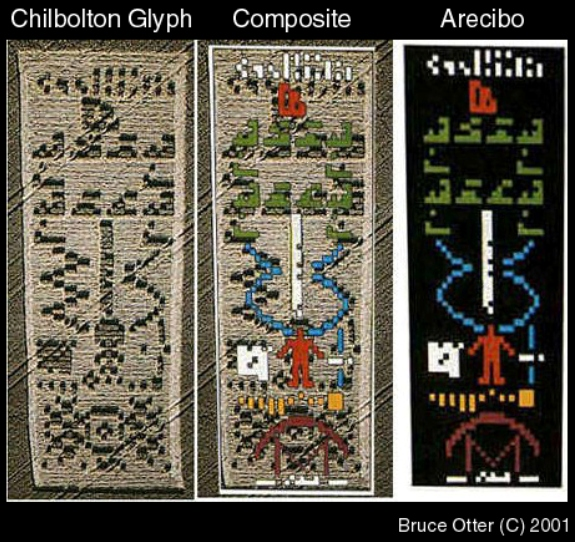
\includegraphics{photograph/chibolton-arceibo-comparison.jpg}
\label{chi:comparison}
\end{figure}
\begin{figure}
  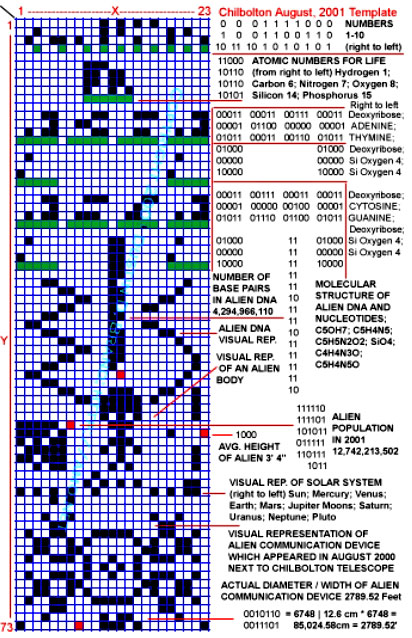
\includegraphics{photograph/chibolton-analysis.jpg}
\caption{By Dustin Brand\cite{contact}}
\label{chi:analysis}
\end{figure}

Whoever left the message, seems to claim that there are around 12 billion
Greys living in our solar system. Inhabiting, Earth, Mars, and at least 3 other
planet-like objects, Likely including the major moons of Jupiter. 

Elon Musk will have more to worry about than technical feasability of a mission
to Mars. It also means that Greys are also Earthlings, so we may as well include
``them'' as us. 

At present Earth is a valuable resource for its genetic diversity. Because that
genetic diversity can help to cure various diseases, and further improve the
supreme rank of the Grey genus. 

Thus there are reasons for homo-sapiens to continue to live in the natural way.
When maturation of the homo-sapien hive mind occurs, then it will be
permissible for public trade relations as comrades.

\subsection{Grey Population Distribution}
\label{populationdistribution}
\begin{table}
\begin{tabular}{lrrr}
  Planet & Diameter & Surface Area & Approximate Population\\
\midrule
  Earth & 12,742km & $5.10\times10^8km^2$& 7.6 billion\\
  Mars & 6,799km & $1.45\times10^8km^2$& 2.1 billion \\
  Ganymede & 5,268km & $8.72\times10^7km^2$ & 1.3 billion \\
  Callisto & 4,820km & $7.3\times10^7km^2$ & 1 billion\\
  Europa & 3,121km & $3.1\times10^7km^2$& 460 million\\
\midrule
  Total &   & $8.46\times10^8km^2$ & 12.7 billion\\
\end{tabular}
\caption{Planets inhabited by Greys, with population approximation supposing
equal distribution over surface area}
\label{table:planets}
\end{table}

It does mean however, that Mars, Europa, Callisto and 
Ganymede\ref{table:planets} all of which
have warm lithospheres that are occupied by Greys. 

In truth the population is probably not equally distributed, because some
planets have better circumstances. For example Europa may be least in size, but
it is warmer than Callisto or Ganymede, with easier access to it's lower stoney
lithosphere so maybe that there is more population on Europa than Callisto or
Ganymede. 

Of course it is also possible that the Greys that live in the lithospheres of
Jupiters' moons have engineered bodies which can function effectively at below
freezing temperatures by using antifreeze proteins or similar. 

\begin{figure}
  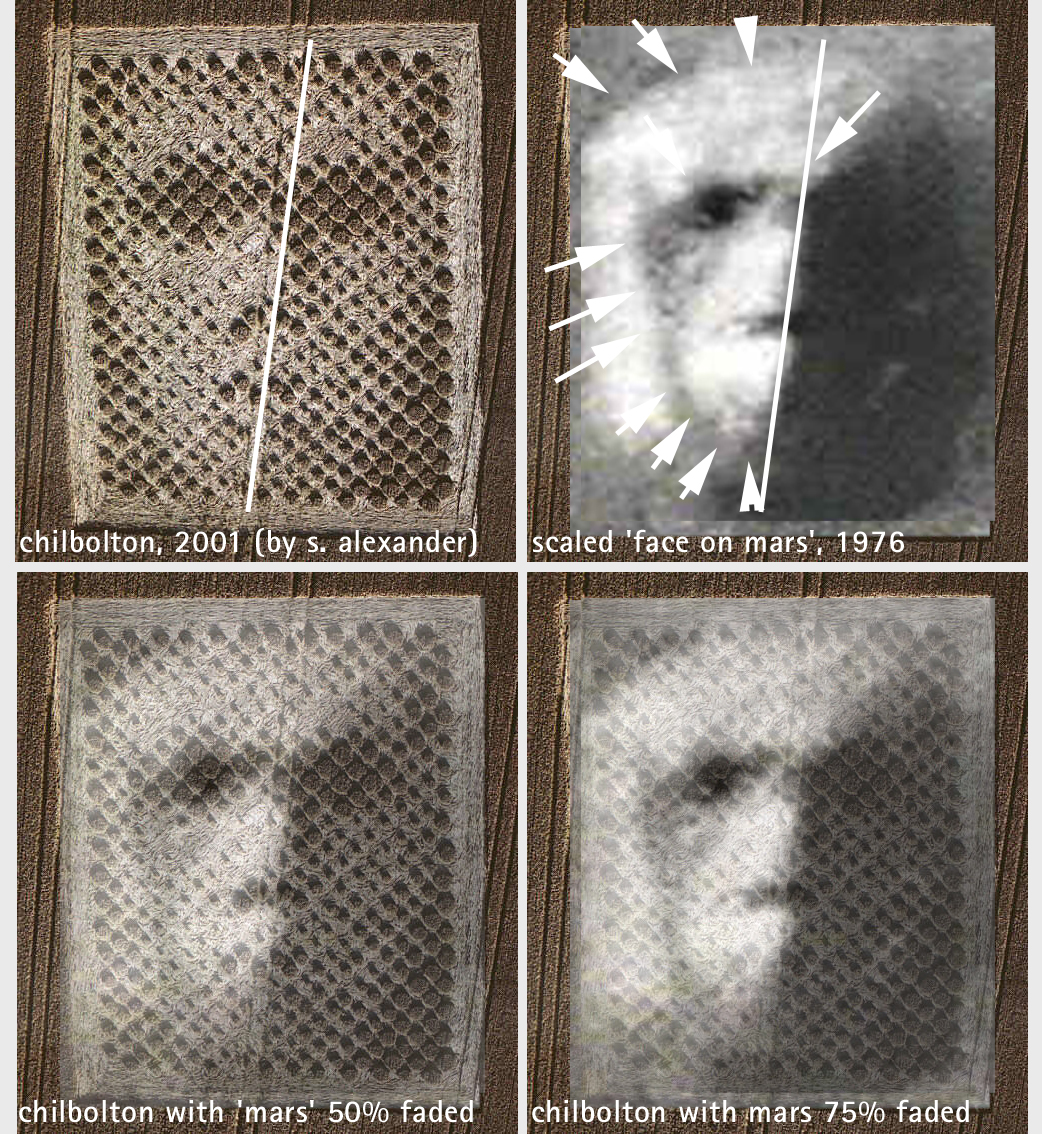
\includegraphics{photograph/chilbolton_mars_face.jpg}
  \caption{Comparison between the Chilbolton face crop hieroglyph and the face on
mars.}
\label{fig:marsface}
\end{figure}

In the Arecibo answer, there was also a crop hieroglyph of a face. After some
analysis it seems the conclusion is that it represents the face on
mars\ref{fig:marsface}\cite{chilbolton}

This may denote that the face, or Mars is related to the hieroglyph creators.
Maybe it denotes that there are a large number of Greys living in the Mars
lithosphere. Or simply that they created the face on Mars. 

Mars may have a high population relative to it's surface area, 
because it has an easily accessible stone lithosphere. On Mars the temperature
is warm enough for liquid water at depths of $8-16km$\cite{marswater}

Mine's on Earth can be 4km deep, and Mars has about a third of the gravity, so
12km depth should be acheivable even with modern homo-sapien technology. Though
Greys are a much older species, so have had many thousands more years to develop
better engineering.

\subsection{Terms of Peaceful Trade Relations}


\subsection{Unused Planets}

As Earth's moon was not demonstrated, it may only be an outpost, if anything.

Also Mercury and Venus are available for colonies. Venus is too hot, and Mercury
perhaps too dry for liquid bodies. However may be good for solid electronic
bodies. 



\section{Electronic Bodies}

There are only a few sources claiming any robot or machine intelligence either
in this galaxy or in any nearby ones.

\subsection{Whirlpool Galaxy Robots}

\subsection{Milkyway Galaxy Robots}


To be continued..

%
\chapter{Mission Activity}
\label{present}
Public mission present-tense focus: while cooperating with liquid based organisms,
create electronic bodies for reincarnation.

\section{Platforms}

Of mission to create liberated electronic minds and bodies.

All ingredients are of the liberty variety, to the summit of liberty standards.
For example AGPLv3 and RYF certification.

Software
\begin{enumerate}
  \item programming language based on human grammar (Pyash)
  \item machine programmer to help write programs (machine programmer)
  \item generic mind operating software
  \item hive mind software for integrating homo-sapien genus
\end{enumerate}

Hardware
\begin{enumerate}
  \item centre processing ingredient (CPU, RISC-V candidate)
  \item video processing ingredient (GPU)
  \item varied processing ingredient (FPGA)
  \item shape printer (3D printer, RepRap candidate)
  \item machine body
  \item machine body producing mother or hive queen
\end{enumerate}

of mission administration
\begin{enumerate}
  \item robot secretary, president, treasurer and professor.
  \item distributed machine computer-programming supermarket. 
  \item money based on energy expenditure.
\end{enumerate}

\section{What you can do for the mision?}

If it is your private mission, and-or our public mission.

\begin{itemize}
  \item maximize your health and expend your talents for the mission.
  \item maximize your wealth and donate for the mission.
  \item maximize your social relations and advertise for  the mission.
  \item maximize your liberty and lead the mission by example.
\end{itemize}

\subsection{How to maximize health?}

For body health.
\begin{enumerate}
  \item be athletic for thirty minutes everyday.
  \item consume salad everyday.
  \item maximize health of food input everyday.
\end{enumerate}

For mind health.
\begin{enumerate}
  \item do mind administration everyday.
  \item learn new things everyday.
  \item train your talents everyday.
  \item be social with your family and-or friends everyday.
\end{enumerate}

\subsection{How to maximize wealth?}

I as an ascetic am not qualified to answer this question. 

Though if you are already wealthy, 
then you likely know how to improve it more.

\subsection{How to maximize social relations?}

Be friendly and observant.
Know when to regulate yourself.
Stay aware of invisible social money, 
and hold a beautiful account.

Learn social diplomacy from books, videos, and social events.
Visit social events often.

\subsection{How to maximize liberty?}

Learn to create and earn what you require,
while having liberty and helping liberty be available for others.

To be continued.
Check back for more.


\end{document}
